\documentclass[24pt, a0paper, portrait, margin=5mm, innermargin=0mm,
               blockverticalspace=0mm, blocktitlewidthratio=0.5, colspace=10mm, 
               subcolspace=0mm]{tikzposter} 

% Change font     
\renewcommand{\familydefault}{\sfdefault}

% LATEX PACKAGES
% --------------
  
\usepackage{graphicx}  % package for inserting images, including .pdf
\usepackage{adjustbox} % package for cropping images
\usepackage{url} % package for url 
\usepackage{wrapfig}
\usepackage{lmodern} %mix italic and bold
\usepackage{hyperref}% for url
\usepackage{authblk}
\usepackage{graphicx} 
\usepackage{caption}
\usepackage{mwe}
\usepackage[absolute]{textpos}
\usepackage{selinput}
\usepackage{multicol}
\usepackage{tikz}

% \usepackage{anyfontsize} %increase overall font size
\SelectInputMappings{%
  Lcaron={Ľ}
}

\definecolor{applegreen}{rgb}{0.55, 0.71, 0.0}
\definecolor{calpolypomonagreen}{rgb}{0.12, 0.3, 0.17}

% TITLE, AUTHORS, INSTITUTE
% -------------------------

\title{\textbf{\parbox{\linewidth}{\centering Reduced \textit{Eimeria} and pinworms loads in hybrid mice of the European house mouse hybrid zone}}}

\author[1,2,*]{\Large Alice~Balard}
\author[1,2]{Victor~Hugo~Jarqu\'{i}n-D\'{i}az}
\author[1]{Jenny~Jost}
\author[3]{Iva~Martincov\'{a}}
\author[3]{{Ľ}udov\'{i}t \v{D}ureje}
\author[3]{Jaroslav~Pi\`alek}
\author[4]{Milo\v{s}~Macholán}
\author[3]{Jo\"{e}lle~Go\"{u}y~de~Bellocq}
\author[3]{Stuart~J.E.~Baird}
\author[1,2]{Emanuel~Heitlinger}

\affil[1]{\large Institute for Biology. Department of Molecular Parasitology. Humboldt University Berlin, Germany}
\affil[2]{\large Leibniz Institute for Zoo and Wildlife Research, Berlin, Germany}
\affil[3]{\large Research Facility Studenec, Institute of Vertebrate Biology, Czech Academy of Sciences, Czech Republic}
\affil[4]{\large Laboratory of Mammalian Evolutionary Genetics, Institute of Animal Physiology and Genetics, Czech Academy of Sciences, Czech Republic}
\affil[*]{\textcolor{black}{contact: alice.cam.balard@gmail.com}\vspace{-4ex}% reduce space
}

\makeatletter
\def\maketitle{\AB@maketitle}
\makeatother

% THEME SETTING
% -------------
\usetheme{Simple}
\colorlet{titlebgcolor}{applegreen}
\colorlet{titlefgcolor}{white}
\colorlet{blocktitlebgcolor}{calpolypomonagreen}
\colorlet{blocktitlefgcolor}{applegreen}

\colorlet{blocktitlebodycolor}{red}



% HEAD
% ----

\begin{document}
\maketitle[linewidth = 2mm]

% Context
% ----

\block{Are hybrid mice more or less susceptible to parasites infection?}
{\Large \begin{itemize}
	   \item Parasite models: 
	    \begin{itemize}
	  		\item \textit{Eimeria} spp., obligate intracellular parasite (Apicomplexa: Coccidia). \textbf{High impact on host health expected}
	  		\item Pinworms \textit{Aspiruluris tetraptera} and \textit{Syphacia obvelata} (Nematoda: Oxyurida). \textbf{Low impact on host health expected}
	    \end{itemize}
	  \item Host model: \textit{Mus musculus domesticus}, \textit{M. m. musculus} and their hybrids
  \end{itemize}
}	

% MATANDMET
% ----

\begin{columns}
  \column{0.3} \block{}{
  
    \begin{tikzfigure}[]
               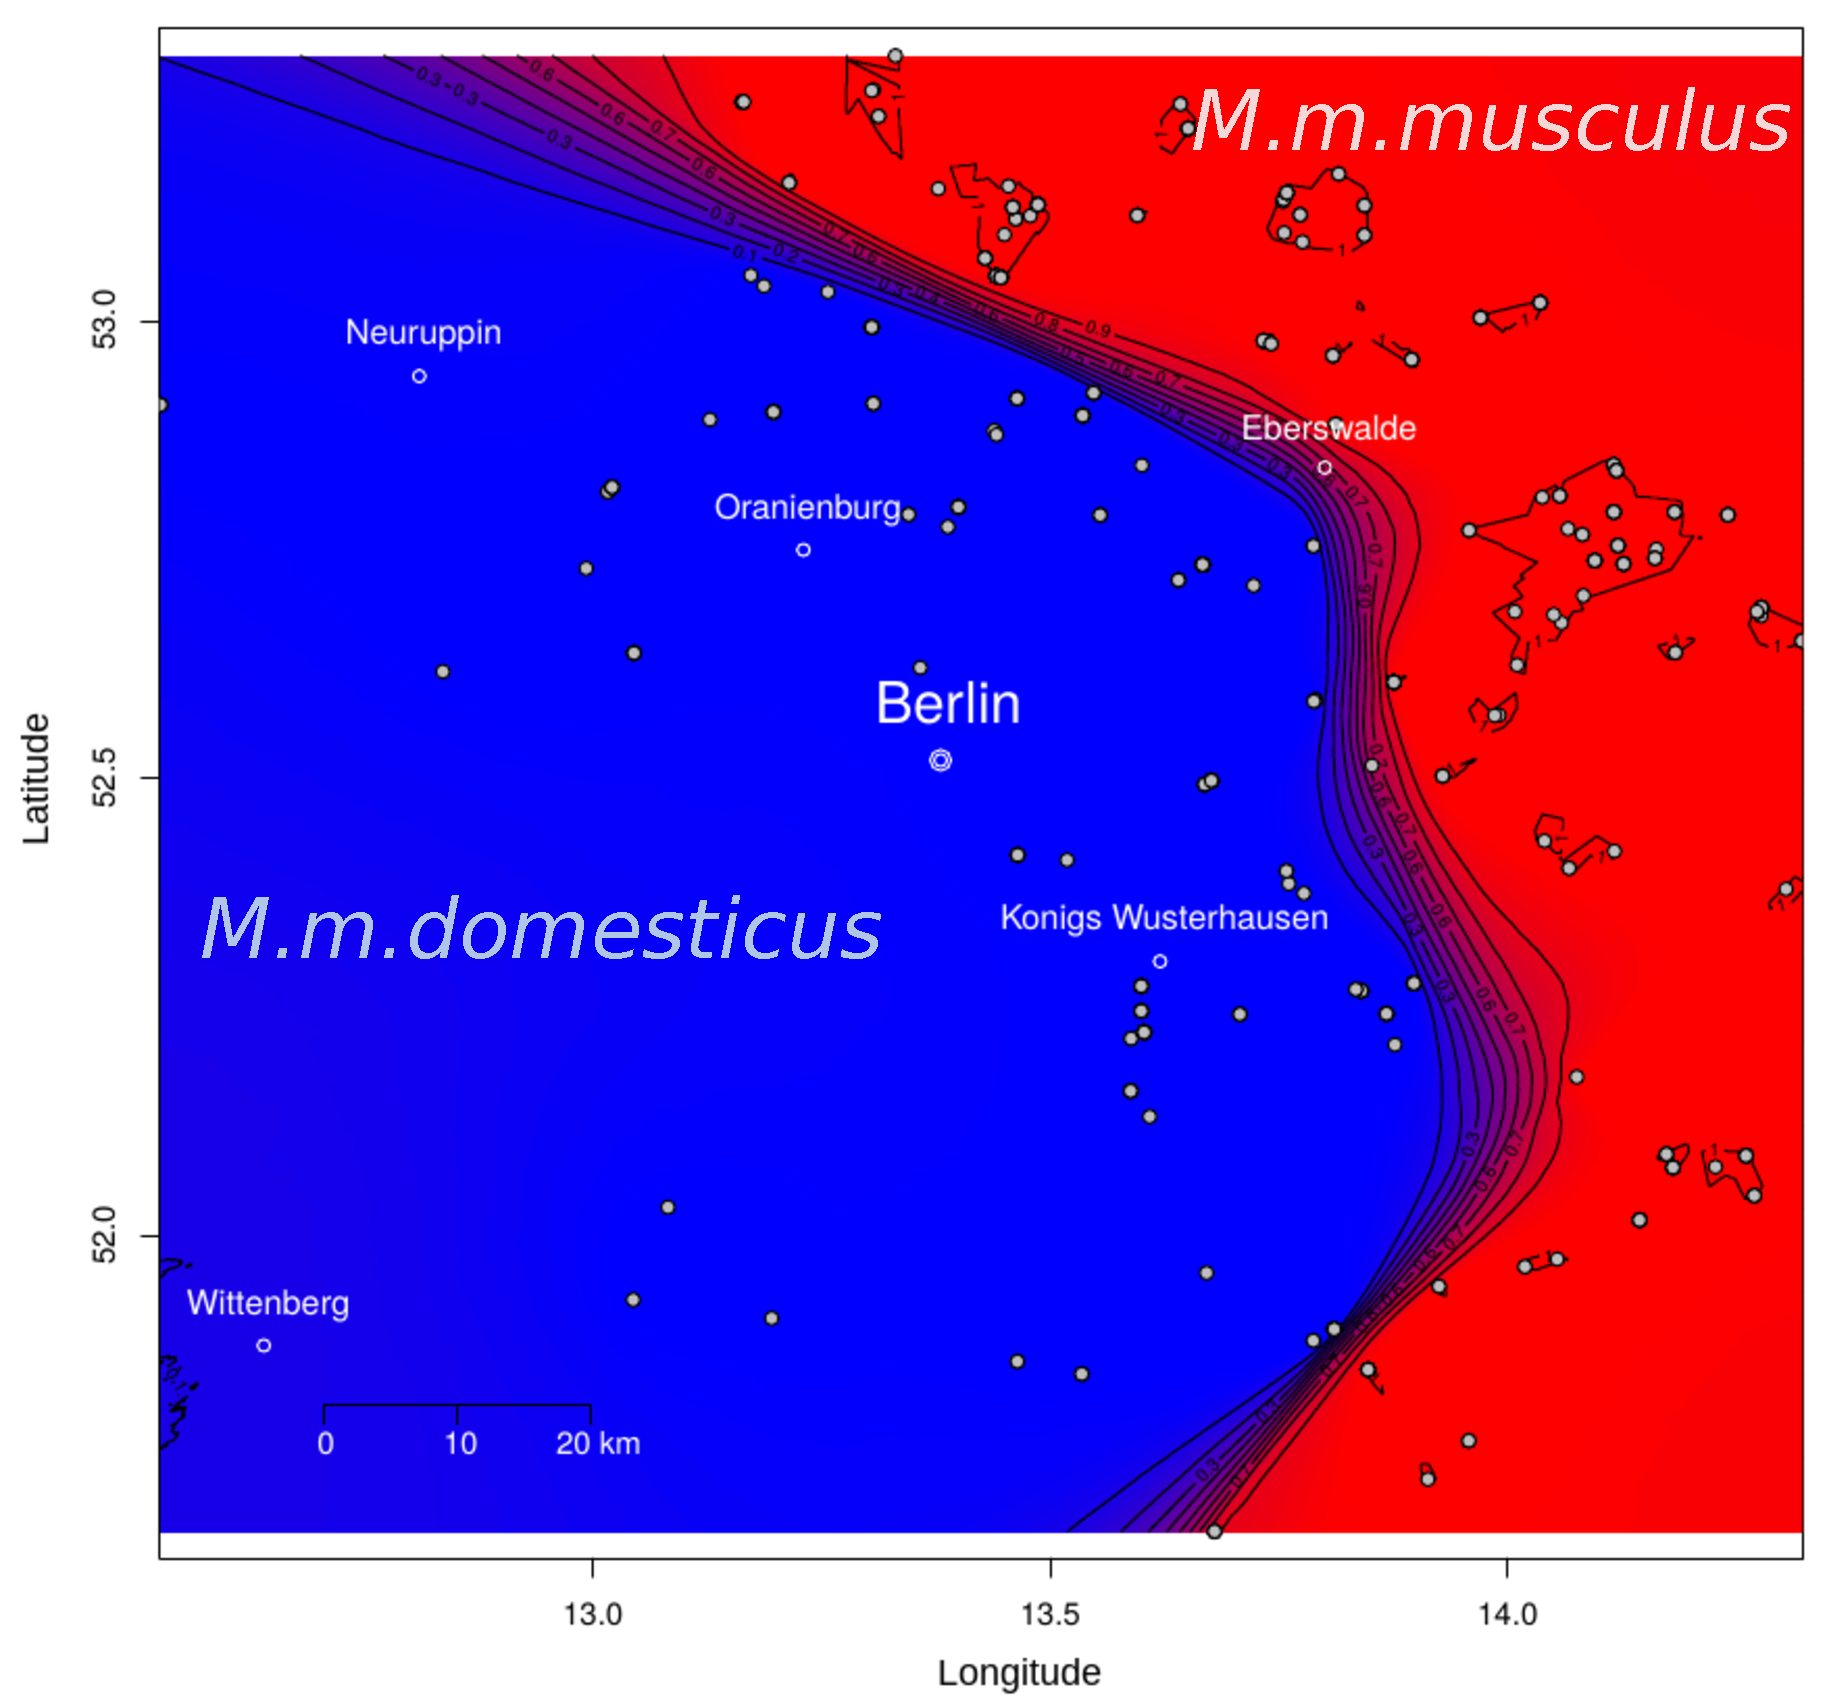
\includegraphics[scale=0.7]{Figure1.pdf}
    \end{tikzfigure}
    }
  \column{0.7} \block{How and where did we do that?}{\Large
    \begin{itemize}
     \item Sampling 660 mice over 4 years in a new transect of the European house mouse hybrid zone
     \item Host genotyping (4-14 diagnostic markers) on a 0 to 1 scale (equal admixture hybrids = 0.5)
     \item \textit{Eimeria} intensity estimated by quantitative PCR, pinworm intensity by count
     \item Modelling of parasite intensity along hybridization index, test hybrid effect by maximum likelihood
     \item Logistic regression presence/absence of parasite in direction of the hybrid zone centre
     \item Body condition = residuals body length/body weight. Modelling of body condition along hybridization index, test hybrid effect by maximum likelihood, test difference between infected/non-infected
      \end{itemize}
  }
  
\end{columns}

% Results: parasite intensity
% -------

% Text and figure Inside the Block 

\begin{columns}\column{0.75}

\block{\textit{Eimeria} spp. and pinworm intensities are lower in hybrids than in parental mice}{
\begin{minipage}[t]{0.5\linewidth}
\Large \centering \textit{Eimeria} \begin{tikzfigure}[] 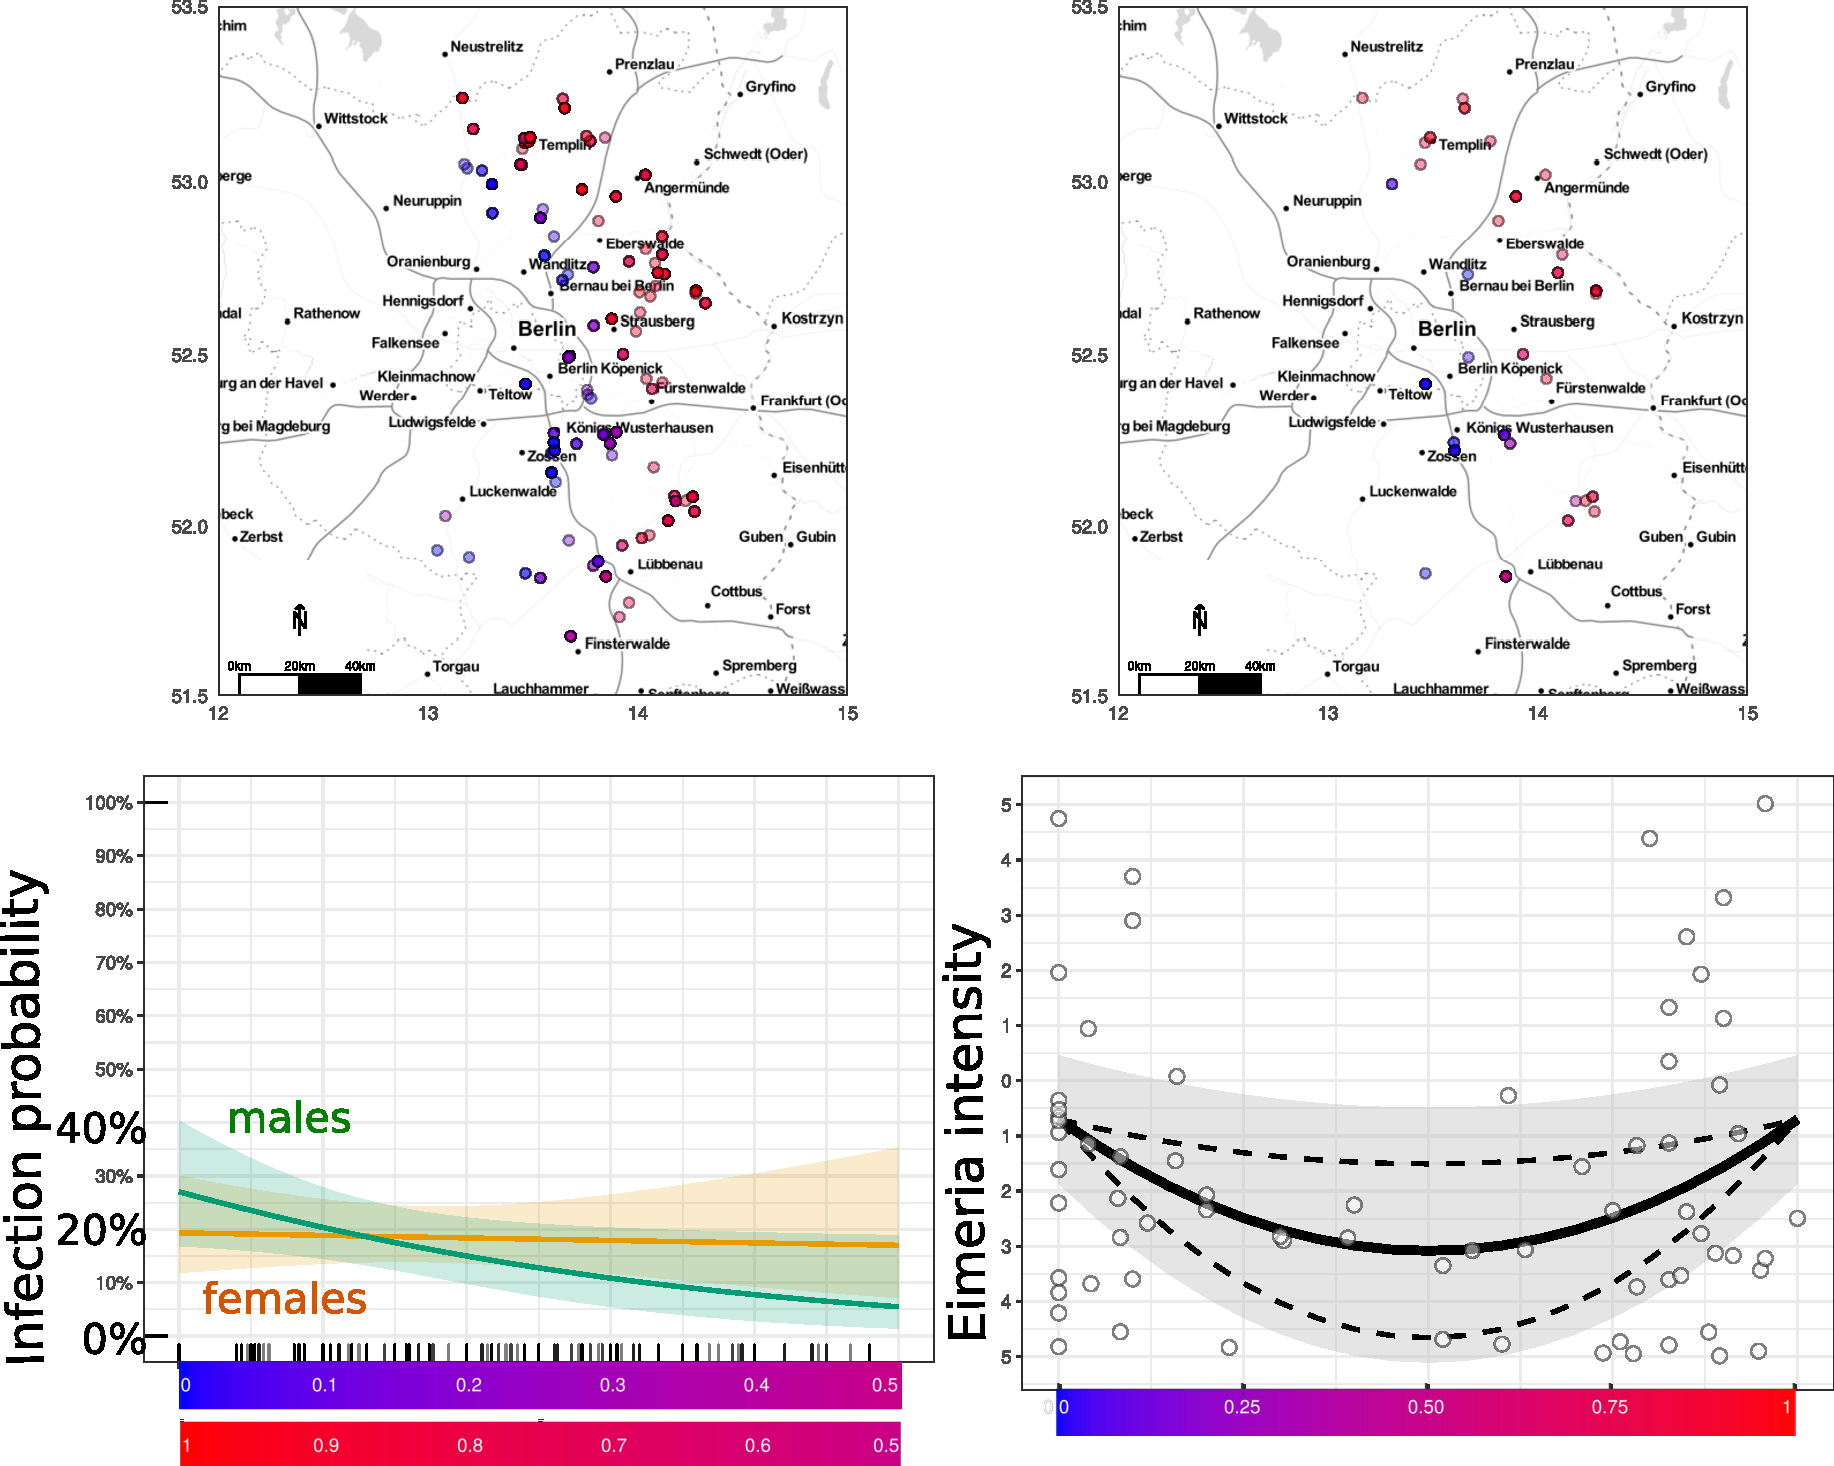
\includegraphics[scale = 0.9]{Figure2.pdf}
  \end{tikzfigure}
\end{minipage}%
\begin{adjustbox}{valign=t}
\begin{minipage}[t]{0.5\linewidth}
\Large \centering Pinworms \begin{tikzfigure}[] 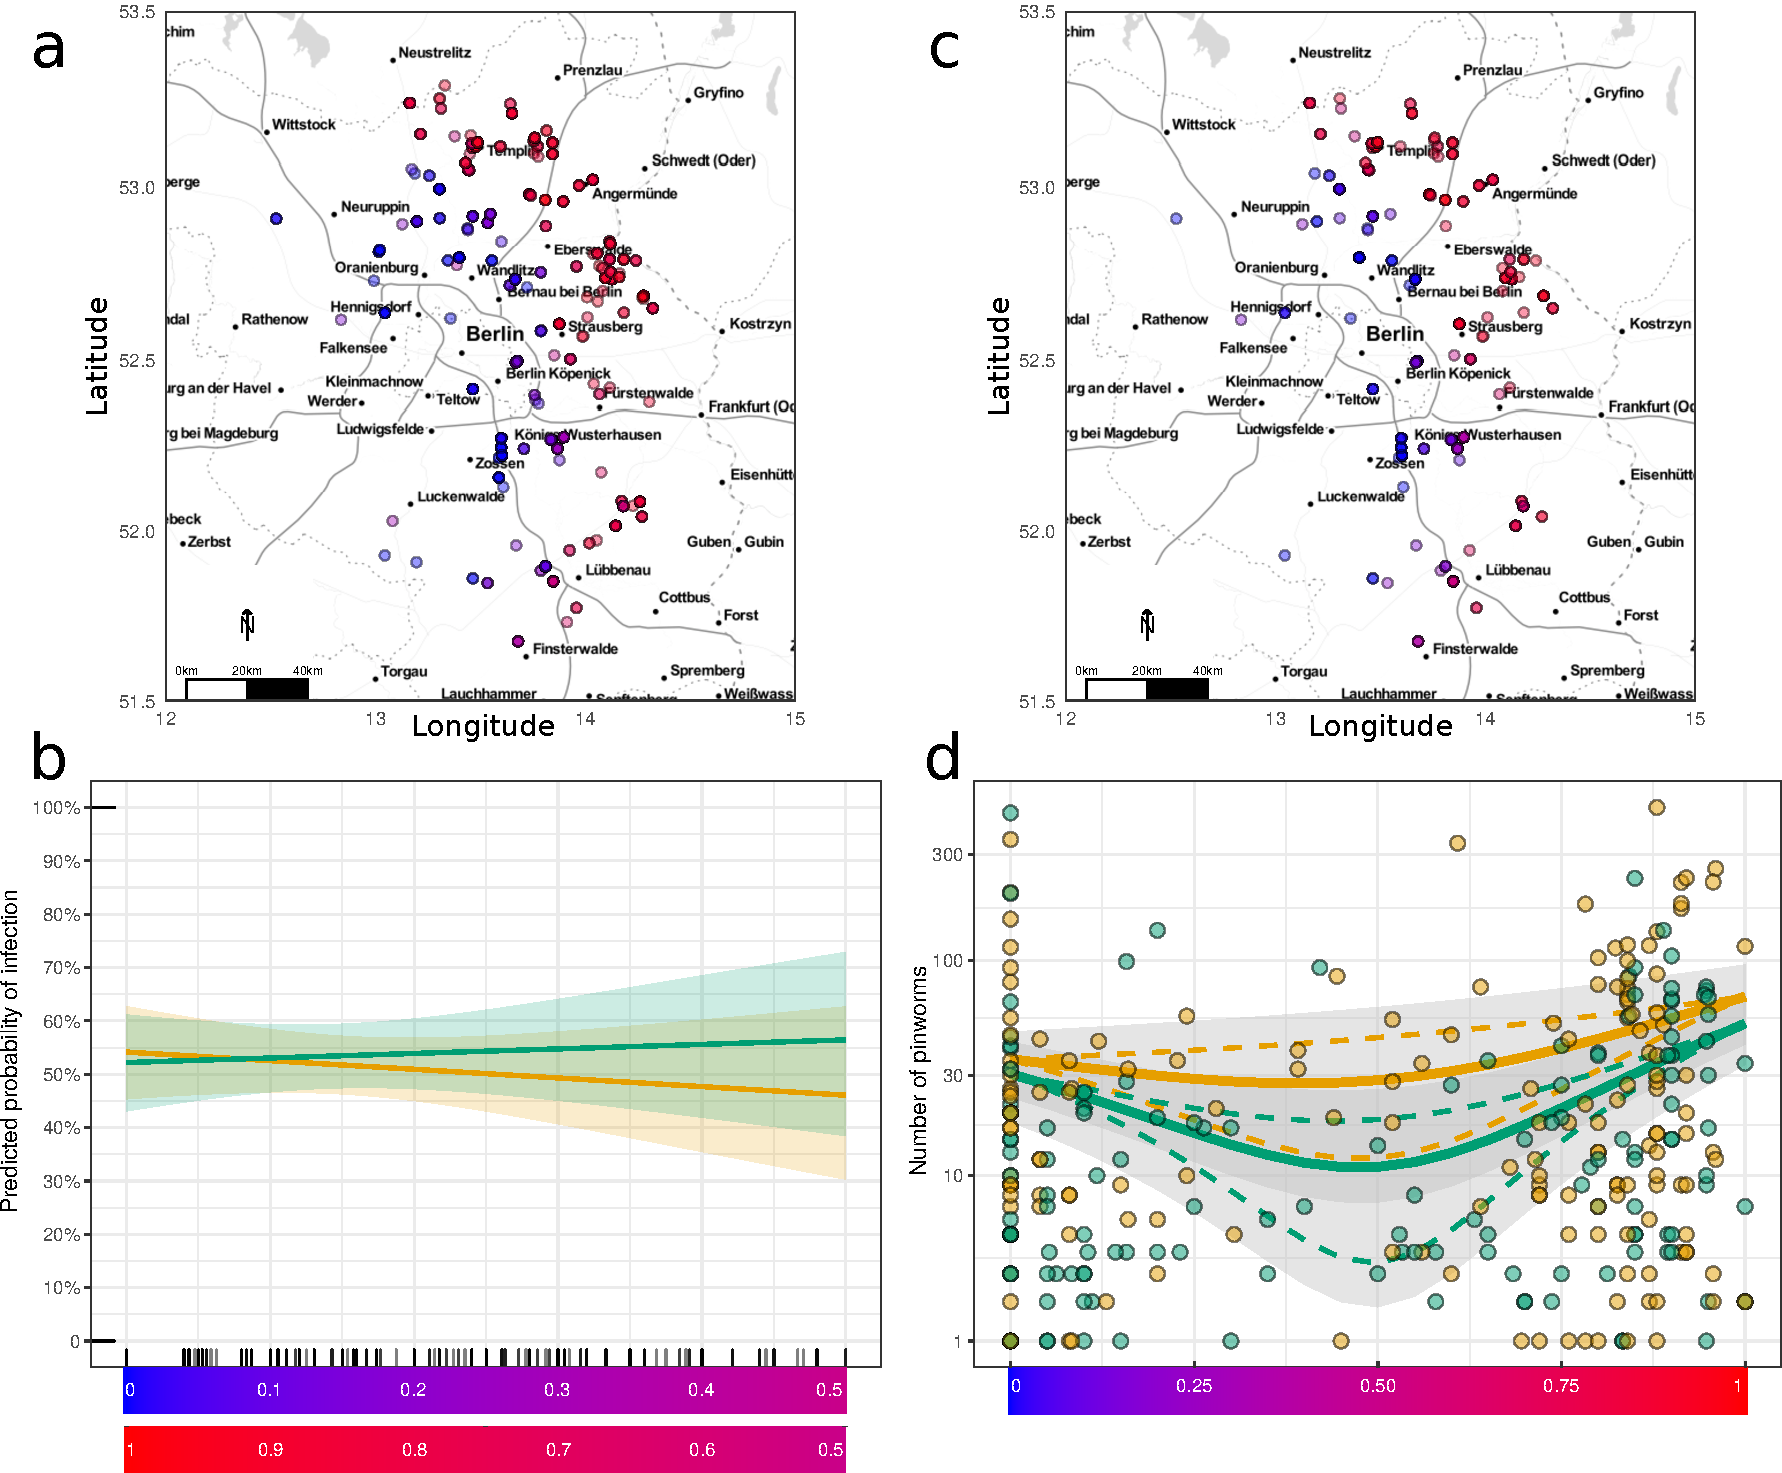
\includegraphics[scale = 0.9]{Figure3.pdf}
  \end{tikzfigure}
\end{minipage}
\end{adjustbox}

}

\column{0.25}\block{}{
\LARGE \centering \textcolor{applegreen}{\textbf{Mouse body condition}} \begin{tikzfigure}[] 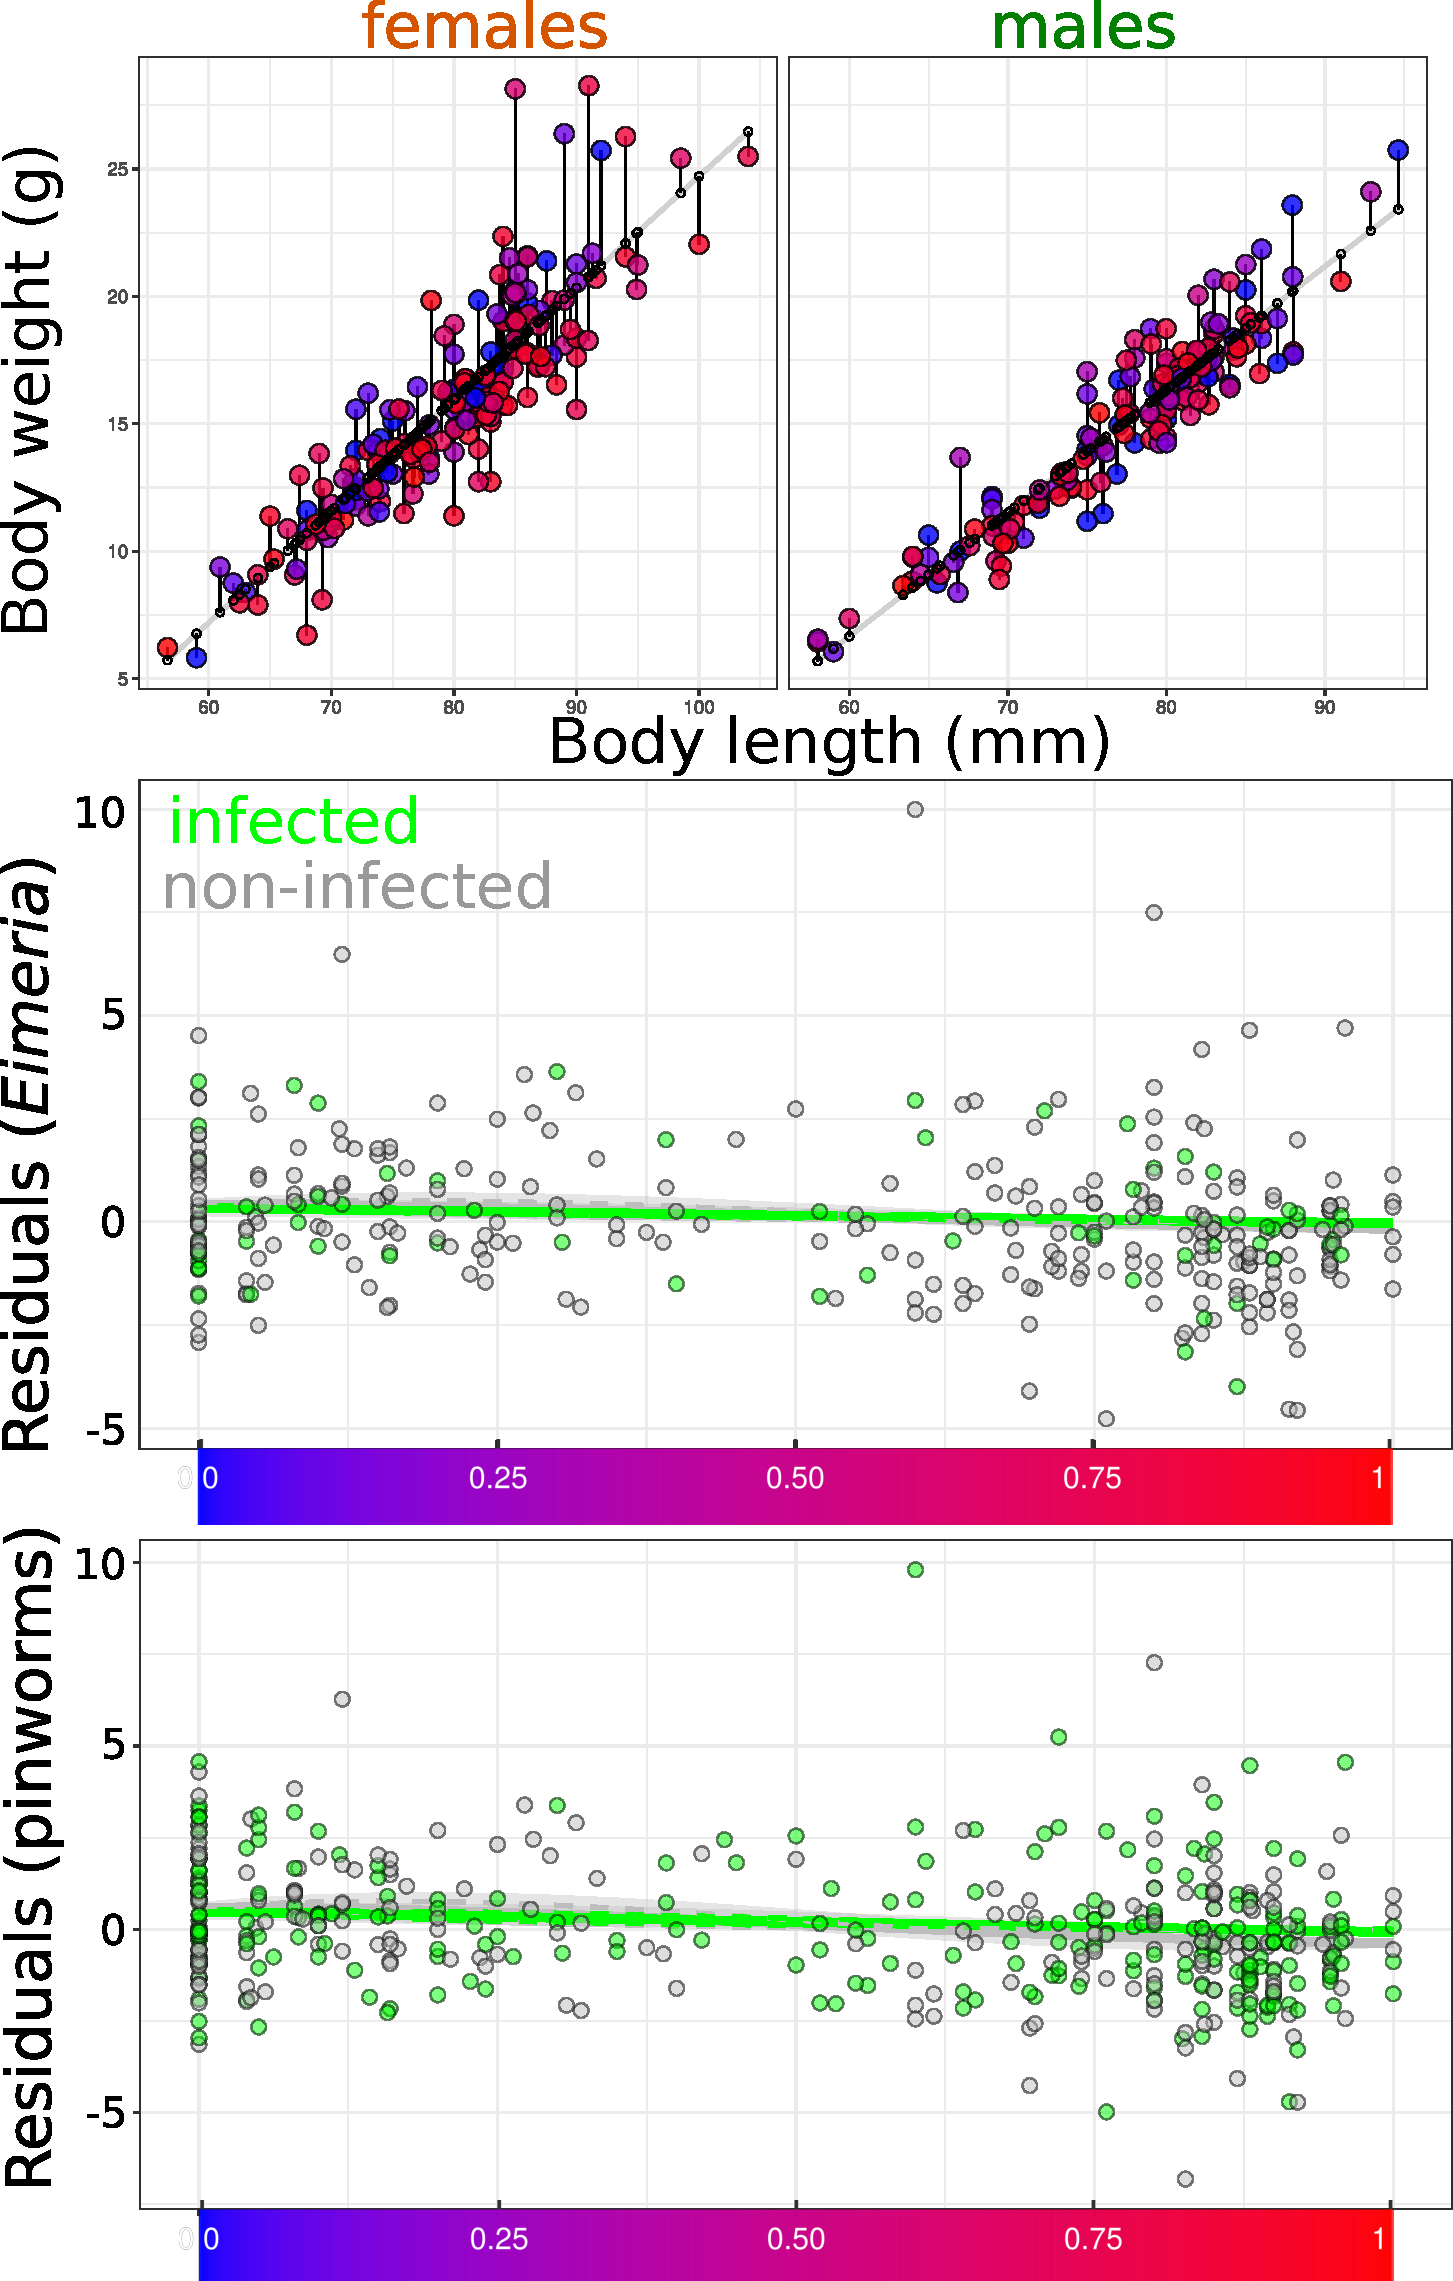
\includegraphics[scale = 0.65]{Figure4.pdf}
  \end{tikzfigure}
}
\end{columns}

\block[bodyoffsety=5cm,titleoffsety=5cm]{}
{  % here increase space
\begin{itemize}
  \item \Large{Lower intensity of both lowly (pinworms) and highly (\textit{Eimeria}) pathogenic parasites in hybrid compared to parental mice}
  \item No indication of lower prevalence in the centre of the hybrid zone
  \item No indication of differential impact of infection on body condition along hybrid gradient
  
\end{itemize}
}


\begin{columns} 
  \column{0.8} 
% PERSPECTIVE
% ----------
\block{What does this mean?}{\Large

\begin{itemize}
  \item Independence of hybrid resistance from the parasite pathogenicity level
  \item Intrinsic components of the host-parasite interaction, instead of ecological and epidemiological factors (e.g. host density troughs), explain intensity reduction in the absence of prevalence reduction
  \item Impact of parasite infection on host health in hybrid zones remains an open question. Differences in host health could contribute as one component to the overall fitness of hybrids
  \item Change to a parasitological perspective: impact of host hybridization on parasites is obvious
\end{itemize}
}
 % REFERENCES
% ----------
  \block{References}{
Balard \textit{et al.} (unpublished) Reduced \textit{Eimeria} and pinworms loads in hybrid mice of the European house mouse hybrid zone \newline
R package used for modelling: Balard, A., and E. Heitlinger. 2019. Alicebalard/parasiteLoad DOI: 10.5281/zenodo.2535547
  }

\column{.2}
   \block[]{}{\LARGE \centering
    \textcolor{applegreen}{\textbf{Funding}}\vspace{-2ex}
    \begin{tikzfigure}[]
    
\includegraphics[scale=1]{acknowledgement.png}
   \end{tikzfigure}}
   
   
\end{columns}

% ----------------
\end{document}
\endinput
%%
%% End of file 
